\begin{figure}[h]
    \centering
    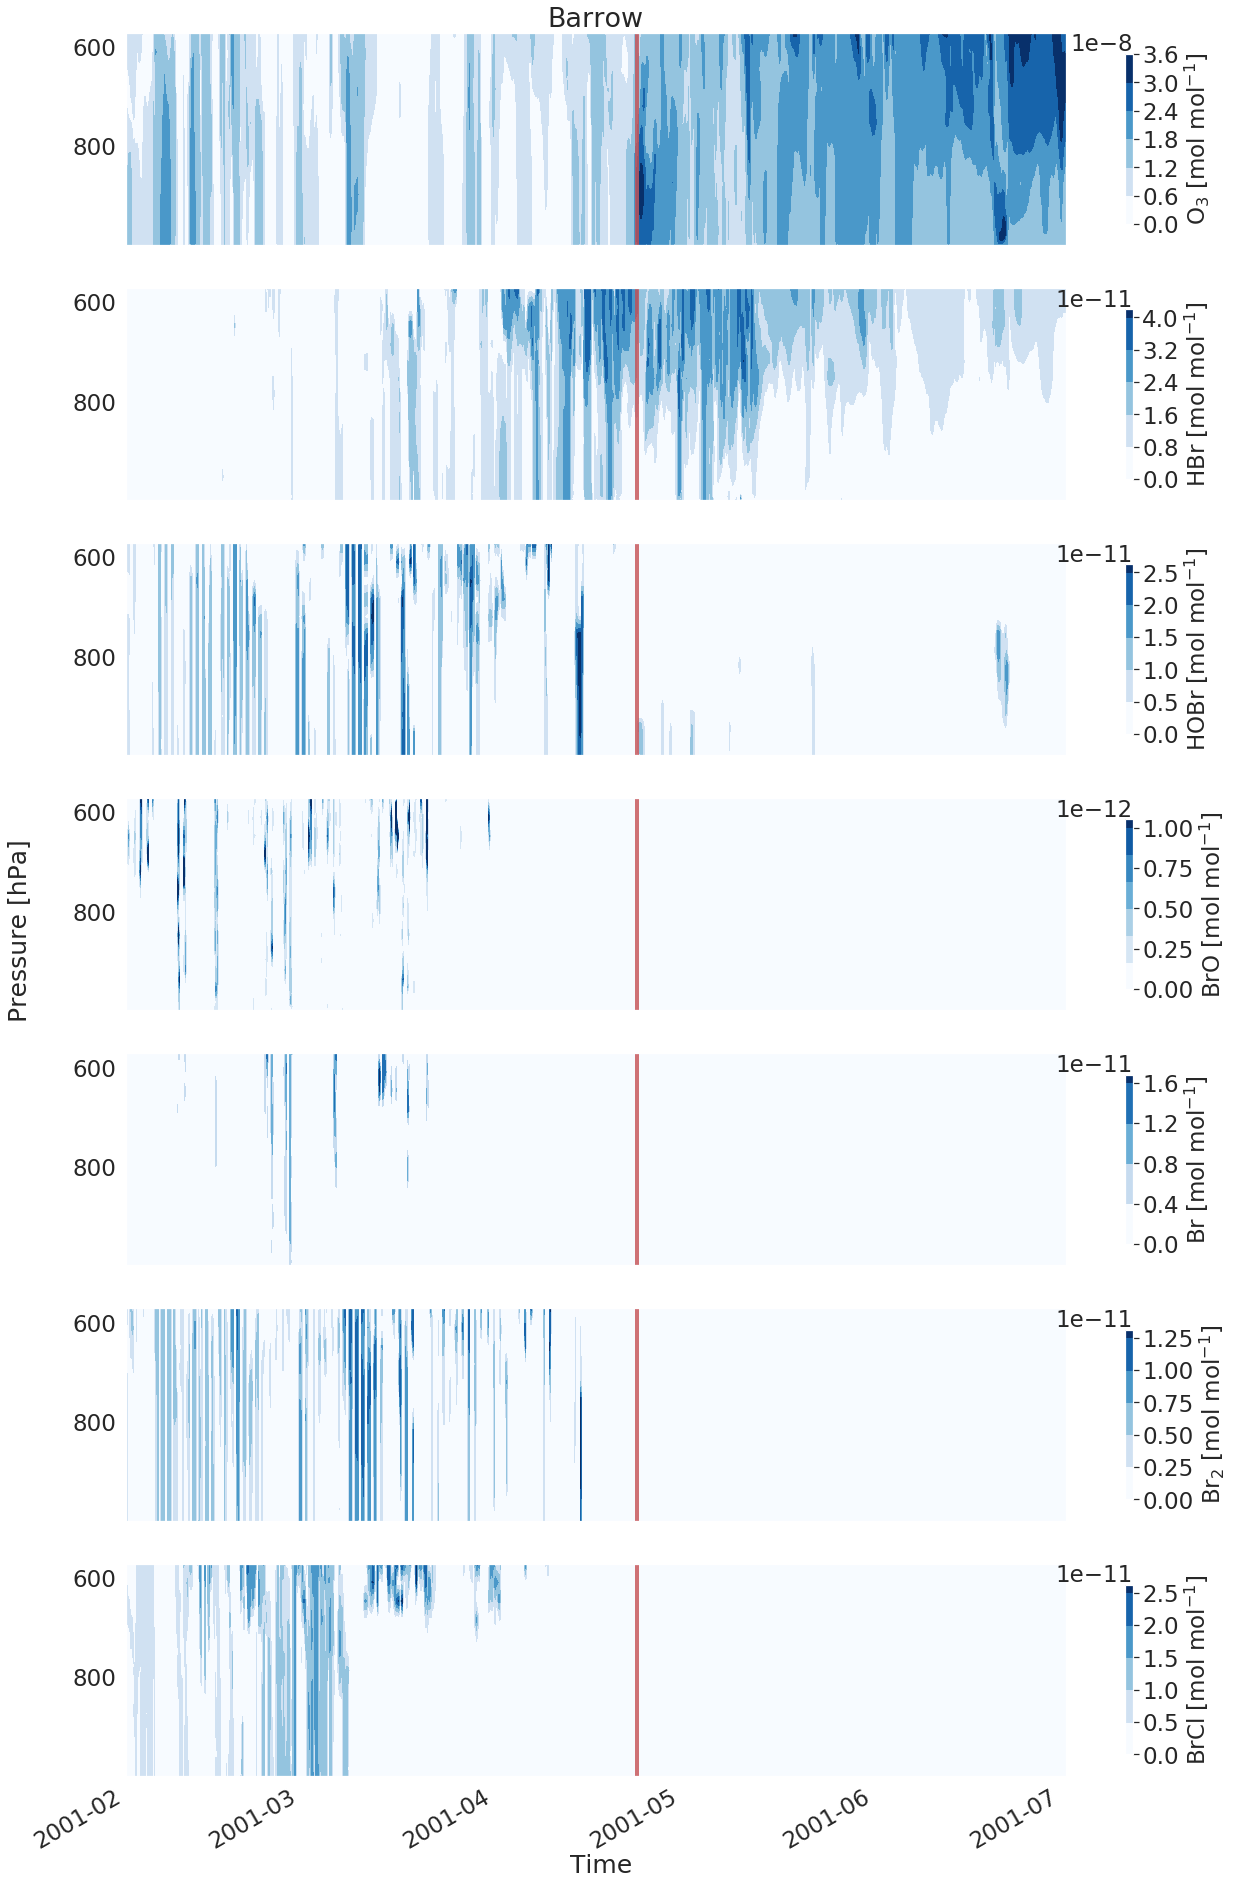
\includegraphics[width=0.8\linewidth]{Chapter6_Results/images/Vert_StationComp_2001/vert_all_species_BRW.png}
    \caption{Mixing ratio ($mol mol^{-1}$) of $\chem{O_3}$, $\chem{HBr}$, $\chem{HOBr}$, $\chem{BrO}$,$\chem{Br}$ and $\chem{Br_2}$ from the station ground level up to $\sim 600 hPa$ at Barrow in Period 1 (left of the red line) and Period 2 (right of the red line) in 2001. \textbf{Note:} the max \chem{BrO} vmr was adjusted down to properly see the maxima}
    \label{fig:vert_BRW}
\end{figure}